\documentclass[]{standalone}
\usepackage[T1]{fontenc}
\usepackage{tikz}
\usepackage{amsmath, amsfonts}
\usepackage{xintexpr}
\usetikzlibrary{arrows, shapes.geometric, calc, positioning, decorations.pathreplacing}

% \makeatletter
% \def\input@path{{./includes/}{./includes/ut/diags/}}
% \makeatother

\tikzstyle{stdText} = [align=center, inner sep=5pt]
\tikzstyle{check} = [stdText, draw, rectangle, rounded corners]
\tikzstyle{action} = [stdText, draw, rectangle, sharp corners, double, dash pattern={on 10pt off 1pt}]
\tikzstyle{ar} = [->, anchor=north, rounded corners, shorten >= 2pt, shorten <= 2pt]
\tikzstyle{label} = [align=center, anchor=center]
\tikzstyle{l2} = [align=left, anchor=west, xshift=-1.5em]
\tikzstyle{lr} = [align=right, anchor=east, xshift=1.5em]
\tikzstyle{lb} = [align=center, anchor=north, yshift=-1em]
\tikzstyle{braceUnder} = [decorate, decoration={brace,amplitude=6pt,mirror,raise=2pt}, line width=.25mm]%
\tikzstyle{braceLeft} = [decorate, decoration={brace,amplitude=6pt,mirror,raise=4pt}, line width=.25mm]%
\tikzstyle{bigText} = [scale=1.5]

\begin{document}%
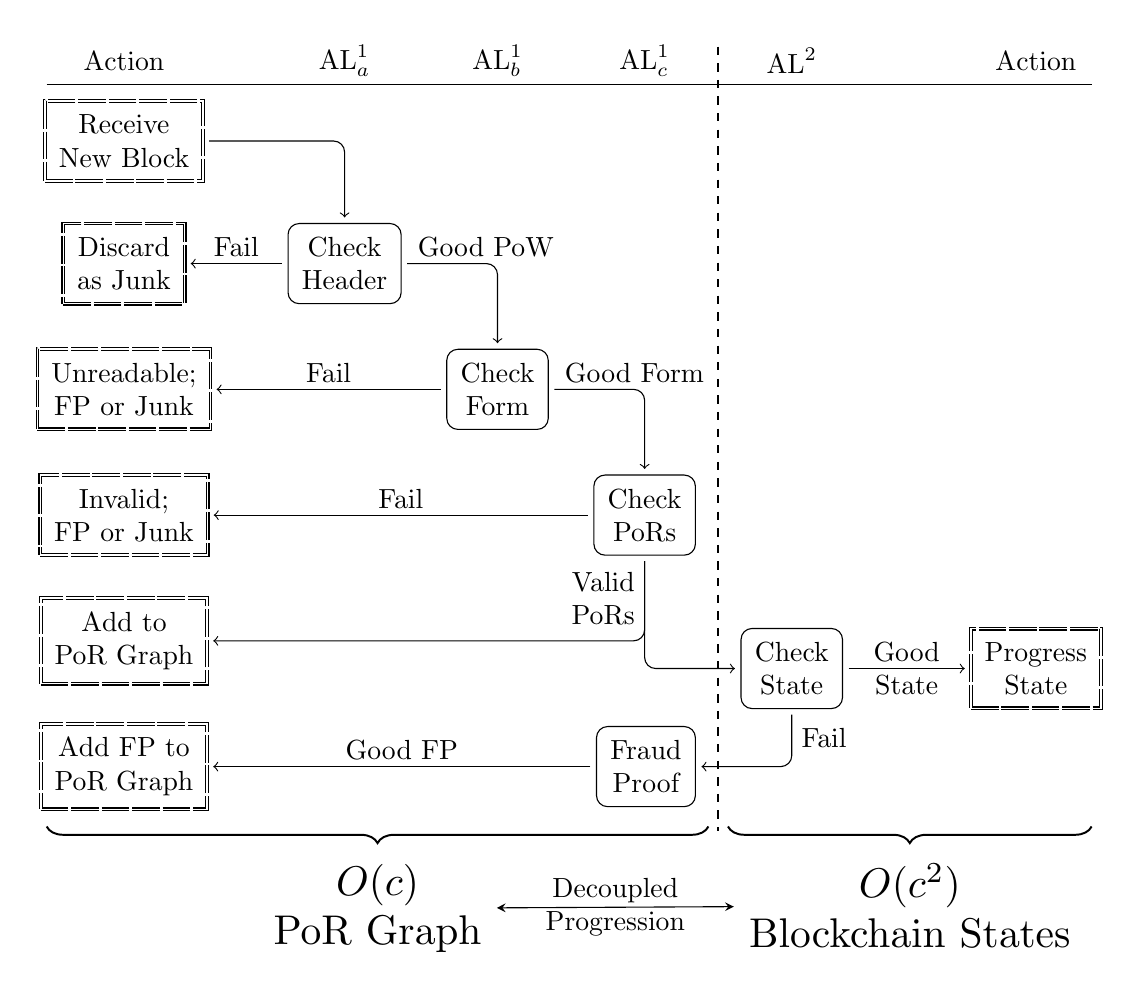
\begin{tikzpicture}[node distance=.8cm]
    % the conditions
    \node (f1) [check] {Check \\ Header};
    \node (f2) [check, below right=of f1] {Check \\ Form};
    \node (f3) [check, below right=of f2] {Check \\ PoRs};
    \node (f4) [check, below right=of f3, yshift=-1em] {Check \\ State};
    \node (f5) [check, below left=of f4, yshift=1em] {Fraud \\ Proof};

    \node (fDone) [action] at ($(f4)!3.1cm!(f4.east)$) {Progress \\ State};
    % \node (start) [xshift=-1.2em] at ($(f1)!2.7!(f1.north west)$) {};

    \node (a1) [action, left = of f1, xshift=-.5cm] {Discard \\ as Junk};
    \node (start) [above left=of f1, yshift=1em] {};
    \node (a2) [action] at (a1 |- f2) {Unreadable; \\ FP or Junk};
    \node (a3) [action] at (a1 |- f3) {Invalid; \\ FP or Junk};
    % \node (a3a) [action] at (a1 |- f3a) {Add to \\ PoR Graph};
    % \node (a4) [action] at (a1 |- f4) {Valid PoRs \\ Link FP if possible};
    \node (a4) [action, yshift=1em] at (a1 |- f4) {Add to \\ PoR Graph};
    \node (a5) [action] at (a1 |- f5) {Add FP to \\ PoR Graph};

    \node (actions) [stdText, yshift=2.9em] at (a1 |- start) {Action};
    \node (p1) [stdText] at (actions -| f1) {$\text{AL}^1_a$};
    \node (p2) [stdText] at (actions -| f2) {$\text{AL}^1_b$};
    \node (p3) [stdText] at (actions -| f3) {$\text{AL}^1_c$};
    \node (p4) [stdText] at (actions -| f4) {$\text{AL}^2$};
    \node (stateAction) [stdText] at (actions -| fDone) {Action};

    \foreach \x in {1,...,3}{
        \draw [ar] (f\x) -- node [label] {Fail \\} (a\x);
    }
    % \draw [ar] (f4) -- node [label] {Fail \\} (a4);

    \foreach \x in {1,...,3}{
        \pgfmathtruncatemacro\y{\x + 1}
        \node (t\x) at (f\x -| f\y) {};
    }

    \node (newBlock) [action] at (start -| actions) {Receive \\ New Block};

    \draw [ar] (newBlock) -- (start -| f1) -- (f1);
    \draw [ar] (f1) -- node [l2] {Good PoW \\} (f1 -| f2) -- (f2);
    \draw [ar] (f2) -- node [l2] {Good Form \\} (f2 -| f3) -- (f3);
    \draw [ar] (f3) -- node [label, anchor=east] {Valid \\ PoRs} (f3 |- a4) -- (a4);
    \draw [ar] (f3) -- (f3 |- f4) -- (f4);
    \draw [ar] (f4) -- node [label, anchor=west, align=left] {Fail} (f4 |- f5) -- (f5);
    \draw [ar] (f4) -- node [label] {Good \\ State} (fDone);
    \draw [ar] (f5) -- node [label] {Good FP\\} (a5);


    % line under headings

    \node (hruleL) [yshift=.0em] at (actions.south west -| a2.west) {};
    % \node (hrRX) at ($(f4)!.5!(fDone)$) {};
    \node (hrRX) at (fDone.east) {};
    \node (hruleR) at (hruleL -| hrRX) {};
    \draw (hruleL) -- (hruleR);

    % division between O(c) and O(c^2)

    \node (divPoint1) at ($(f3)!.5!(f4)$) {};
    \node (divPointT) at (divPoint1 |- actions.north) {};
    \node (divPointB) [yshift=-.4em] at (divPoint1 |- a5.south) {};
    \node (BR) at (fDone.east |- divPointB) {};
    \node (TR) at (BR |- divPointT) {};
    \draw [thick, dashed] (divPointT) -- (divPointB.south);

    % \node (BL1) at (BR -| f1.west) {};
    \node (BL1) at (BR -| hruleL) {};

    \draw [braceUnder] (BL1) -- node (complexity1) [lb, bigText] {$O(c)$ \\ PoR Graph} (divPointB);
    \draw [braceUnder] (divPointB) -- node (complexity2) [lb, bigText] {$O(c^2)$ \\ Blockchain States} (BR);
    \draw [stealth-stealth] (complexity1) -- node [label] {Decoupled \\ Progression} (complexity2);

    % \draw [braceLeft] (a3.north west) -- node [label, anchor=south, rotate=90] {DA Consensus\\} (a4.south west);
    % \draw [braceLeft] (a5.north west) -- node [label, anchor=south, yshift=-1em, rotate=90] {EC Consensus\\} (a5.south west);
\end{tikzpicture}%
\end{document}%
